\documentclass[12pt]{article}

%\usepackage[cm]{fullpage}
\setlength{\topmargin}{-1in}
\setlength{\oddsidemargin}{-0.25in}
\setlength{\evensidemargin}{-0.25in}
\setlength{\textwidth}{7in}
\setlength{\textheight}{10in}


\usepackage{tikz}
\usetikzlibrary{backgrounds}
\usetikzlibrary{arrows,arrows.meta,matrix}
\usetikzlibrary{decorations}
\usetikzlibrary{animations}
\usetikzlibrary{tikzmark,calc}
\usetikzlibrary{bending, positioning}
\usetikzlibrary{3d}
% do not indent outermost itemize environ
%\setlength{\leftmargini}{0in}
%
%\usepackage{hyperref}
\usepackage{multicol}
\usepackage{graphicx}
\usepackage{amsmath}
\usepackage{amssymb}
\usepackage{mathrsfs}
\newcommand{\ds}{\displaystyle}
\renewcommand{\Re}{\mbox{Re}}
\renewcommand{\Im}{\mbox{Im}}
\newcommand{\Arg}{\mbox{Arg}}
\newcommand{\Ln}{\mbox{Ln}}
\renewcommand{\L}{\mathscr{L}}
%\renewcommand{\arraystretch}{1.5}
\usepackage{enumitem}
\usepackage{hyperref}
\usepackage{amssymb}
\usepackage{amsmath}
\usepackage{multicol}
\usepackage{array, latexsym}
\usepackage{times}
\usepackage{time}
\usepackage{subfigure}
\usepackage{graphics}
\usepackage{graphicx}
\usepackage{epstopdf}
\usepackage[T1]{fontenc}
\usepackage{setspace}
\newcommand{\To}{\Rightarrow}
\newcommand{\del}{\nabla}
\newcommand{\R}{\mathbb{R}}
\newcommand{\C}{\mathcal{C}}
\newcommand{\N}{\mathcal{N}}
\newcommand{\A}{\mathcal{A}}
\renewcommand{\O}{\mathcal{O}}
% \renewcommand{\N}{\mathbb{N}}
\newcommand{\ben}{\begin{enumerate}}
\newcommand{\een}{\end{enumerate}}
\newcommand{\eps}{\varepsilon}
\renewcommand{\epsilon}{\varepsilon}
\newcommand{\p}{\partial}
\newcommand{\<}{\langle}
\renewcommand{\>}{\rangle}
\renewcommand{\subset}{\subseteq}
\newcommand{\cont}{\Rightarrow \Leftarrow}
\newcommand{\back}{\backslash}
\newcommand{\norm}[1]{\|{#1}\|}
\newcommand{\abs}[1]{|{#1}|}
\newcommand{\ip}[1]{\langle{#1}\rangle}
\newcommand{\m}[1]{{\mathbf{#1}}}
\newcommand{\sts}{\m{S}^\textrm{T}\m{S}}
\newcommand{\rank}{\textrm{rank}}
\newcommand{\X}{\mathcal{X}}
\newcommand{\Y}{\mathcal{Y}}
\renewcommand{\L}{\mathscr{L}}
\def\ds{\displaystyle}
\def\d{\partial}

\def\plottingAxes{
	\begin{tikzpicture}[samples=100, scale=1.2]

		% === figure/domain/tick bounds ===
		\def\tmin{-3.0}	\def\tmax{3.1}
		\def\ymin{-3.0}	\def\ymax{3.1}
		\def\tticks{-3, -2, -1, 1, 2, 3}
		\def\yticks{-3, -2, -1, 1, 2, 3}

		% === Axes ===
		\draw[->] (\tmin	,0		) -- (\tmax	,0		);
		\draw[->] (0		,\ymin	) -- (0		,\ymax	);
		% \node[font=\small, below] at (\tmax - 0.1	, 0) {$t$};

		% === Tick marks/numeric labels ===
		\foreach \t in \tticks {
			\draw[gray]	(\t,0.1) -- (\t,-0.1);					% t ticks
			\node[below, font=\small] at (\t,-0.08) {\t};	% t labels
			
		}
		\foreach \y in \yticks {
			\draw[gray]	(0.1,\y) -- (-0.1,\y);				% y ticks
			\node[right, font=\small] at (0,\y) {\y};	% y labels
		}
		\draw[very thin,color=lightgray] (\tmin,\ymin) grid (\tmax,\ymax);	
	\end{tikzpicture}
}

\def\slopefieldA{
	\begin{tikzpicture}[declare function={f(\x,\y)=\y*\y;}, scale=1.32]

		\pgfkeys{/pgf/number format/.cd,
			fixed,
			precision=0
		}
		\def\tmin{-2.5} \def\tmax{2.5}
		\def\ymin{-2.5} \def\ymax{2.5}
		\def\tmargin{0.5} % extra space around the grid
		\def\ymargin{0.5} % extra space around the grid
		\def\nt{8}  \def\ny{8}
		\def\arrowscale{0.5} % length of slope arrows

		% stepsize along t-axis and y-axis
		\pgfmathsetmacro{\tL}{\tmin + \tmargin}
		\pgfmathsetmacro{\tR}{\tmax - \tmargin}
		\pgfmathsetmacro{\yL}{\ymin + \ymargin}
		\pgfmathsetmacro{\yR}{\ymax - \ymargin}
		\pgfmathsetmacro{\tstep}{(\tR-\tL)/\nt}
		\pgfmathsetmacro{\ystep}{(\yR-\yL)/\ny}

		% Draw grid lines
		\foreach \i in {0,...,\nt} {
			\pgfmathsetmacro{\tk}{\tL + \i * \tstep}
			\draw[thin, gray!50] (\tk, \ymin) -- (\tk, \ymax);
		}
		\foreach \j in {0,...,\ny} {
			\pgfmathsetmacro{\yk}{\yL + \j * \ystep}
			\draw[thin, gray!50] (\tmin, \yk) -- (\tmax, \yk);
		}

		% Axes
		\draw[->] (\tmin, 0) -- (\tmax+0.6, 0) node[xshift=-0.1cm, below] {$t$};
		\draw[->] (0, \ymin) -- (0, \ymax+0.6) node[yshift=-0.1cm, left] {$y$};

		% Bounding box
		\draw[gray!50] (\tmin,\ymin) rectangle (\tmax,\ymax);

		% Tick marks and labels on t-axis
		\foreach \t in {\tL,...,\tR} {
			\pgfmathparse{\t < 0}
			\ifnum\pgfmathresult=1	 % shift negative ticks
				\draw (\t,\ymin-0.1) -- (\t,\ymin+0.1)
				node[font=\small, below, xshift=-0.15cm, yshift=-0.1cm] {\pgfmathprintnumber{\t}};
			\else
				\draw (\t,\ymin-0.1) -- (\t,\ymin+0.1)
				node[font=\small, below, yshift=-0.1cm] {\pgfmathprintnumber{\t}};
			\fi
		}

		% Tick marks and labels on y-axis
		\foreach \y in {\yL,...,\yR}
			\draw (\tmin-0.1,\y) -- (\tmin+0.1,\y)
			node[font=\small, left, xshift=-0.1cm] {\pgfmathprintnumber{\y}};

		% Title
		%\node[above, font=\small\bfseries] at (current bounding box.north) 
		%	{Slope field for \quad $y' = x + y$};

		% slope field: just draw a vector at each point
		\foreach \i in {0,...,\nt}
		\foreach \j in {0,...,\ny}{

			\pgfmathsetmacro{\tpt}{\tL + \i * \tstep}
			\pgfmathsetmacro{\ypt}{\yL + \j * \ystep}
			
			\pgfmathsetmacro{\slope}{f(\tpt,\ypt)}

			% Normalize direction vector (1, slope) to fixed length
			\pgfmathsetmacro{\len}{sqrt(1 + (\slope)^2)}
			\pgfmathsetmacro{\dt}{\arrowscale / \len}
			\pgfmathsetmacro{\dy}{\arrowscale * \slope / \len}

			%\draw[teal!90, -stealth, line width=1.1pt, shift={(\tpt,\ypt)}] (-0.5*\dt, -0.5*\dy) -- (0.5*\dt, 0.5*\dy);
			\draw[teal!95, line width=1.1pt, shift={(\tpt,\ypt)}] (-0.5*\dt, -0.5*\dy) -- (0.5*\dt, 0.5*\dy);
			\draw[fill=white!50] (\tpt,\ypt) circle (0.8pt);

		}

	\end{tikzpicture}
}

\def\slopefieldB{
	\begin{tikzpicture}[declare function={f(\x,\y)=\x/\y;}, scale=1.32]

		\pgfkeys{/pgf/number format/.cd,
			fixed,
			precision=0
		}
		\def\tmin{-2.5} \def\tmax{2.5}
		\def\ymin{-2.5} \def\ymax{2.5}
		\def\tmargin{0.5} % extra space around the grid
		\def\ymargin{0.5} % extra space around the grid
		\def\nt{8}  \def\ny{8}
		\def\arrowscale{0.5} % length of slope arrows

		% stepsize along t-axis and y-axis
		\pgfmathsetmacro{\tL}{\tmin + \tmargin}
		\pgfmathsetmacro{\tR}{\tmax - \tmargin}
		\pgfmathsetmacro{\yL}{\ymin + \ymargin}
		\pgfmathsetmacro{\yR}{\ymax - \ymargin}
		\pgfmathsetmacro{\tstep}{(\tR-\tL)/\nt}
		\pgfmathsetmacro{\ystep}{(\yR-\yL)/\ny}

		% Draw grid lines
		\foreach \i in {0,...,\nt} {
			\pgfmathsetmacro{\tk}{\tL + \i * \tstep}
			\draw[thin, gray!50] (\tk, \ymin) -- (\tk, \ymax);
		}
		\foreach \j in {0,...,\ny} {
			\pgfmathsetmacro{\yk}{\yL + \j * \ystep}
			\draw[thin, gray!50] (\tmin, \yk) -- (\tmax, \yk);
		}

		% Axes
		\draw[->] (\tmin, 0) -- (\tmax+0.6, 0) node[xshift=-0.1cm, below] {$t$};
		\draw[->] (0, \ymin) -- (0, \ymax+0.6) node[yshift=-0.1cm, left] {$y$};

		% Bounding box
		\draw[gray!50] (\tmin,\ymin) rectangle (\tmax,\ymax);

		% Tick marks and labels on t-axis
		\foreach \t in {\tL,...,\tR} {
			\pgfmathparse{\t < 0}
			\ifnum\pgfmathresult=1	 % shift negative ticks
				\draw (\t,\ymin-0.1) -- (\t,\ymin+0.1)
				node[font=\small, below, xshift=-0.15cm, yshift=-0.1cm] {\pgfmathprintnumber{\t}};
			\else
				\draw (\t,\ymin-0.1) -- (\t,\ymin+0.1)
				node[font=\small, below, yshift=-0.1cm] {\pgfmathprintnumber{\t}};
			\fi
		}

		% Tick marks and labels on y-axis
		\foreach \y in {\yL,...,\yR}
			\draw (\tmin-0.1,\y) -- (\tmin+0.1,\y)
			node[font=\small, left, xshift=-0.1cm] {\pgfmathprintnumber{\y}};

		% Title
		%\node[above, font=\small\bfseries] at (current bounding box.north) 
		%	{Slope field for \quad $y' = x + y$};

		% slope field: just draw a vector at each point
		\foreach \i in {0,...,\nt}
		\foreach \j in {0,...,\ny}{

			\pgfmathsetmacro{\tpt}{\tL + \i * \tstep}
			\pgfmathsetmacro{\ypt}{\yL + \j * \ystep}
			
			\pgfmathparse{\ypt != 0} % avoid division by zero
			\ifnum\pgfmathresult=1
				\pgfmathsetmacro{\slope}{f(\tpt,\ypt)}

				% Normalize direction vector (1, slope) to fixed length
				\pgfmathsetmacro{\len}{sqrt(1 + (\slope)^2)}
				\pgfmathsetmacro{\dt}{\arrowscale / \len}
				\pgfmathsetmacro{\dy}{\arrowscale * \slope / \len}

				%\draw[teal!90, -stealth, line width=1.1pt, shift={(\tpt,\ypt)}] (-0.5*\dt, -0.5*\dy) -- (0.5*\dt, 0.5*\dy);
				\draw[teal!95, line width=1.1pt, shift={(\tpt,\ypt)}] (-0.5*\dt, -0.5*\dy) -- (0.5*\dt, 0.5*\dy);
				\draw[fill=white!50] (\tpt,\ypt) circle (0.8pt);
			\else
				% do nothing (skip this point)
			\fi

		}

	\end{tikzpicture}
}

\def\slopefieldC{
	\resizebox{15cm}{9cm}{%
	\begin{tikzpicture}[declare function={f(\x,\y)=\y*\y;}, scale=1]

		\pgfkeys{/pgf/number format/.cd,
			fixed,
			precision=1
		}
		\def\tmin{-2.5} \def\tmax{2.5}
		\def\ymin{-2.5} \def\ymax{2.5}
		\def\tmargin{0.5} \def\ymargin{0.5} % extra space around the grid
		\def\nt{12}  \def\ny{10}
		\def\arrowscale{0.3} % length of slope arrows

		% stepsize along t-axis and y-axis
		\pgfmathsetmacro{\tL}{\tmin + \tmargin}
		\pgfmathsetmacro{\tR}{\tmax - \tmargin}
		\pgfmathsetmacro{\yL}{\ymin + \ymargin}
		\pgfmathsetmacro{\yR}{\ymax - \ymargin}
		\pgfmathsetmacro{\tstep}{(\tR-\tL)/\nt}
		\pgfmathsetmacro{\ystep}{(\yR-\yL)/\ny}

		% Draw grid lines
		\foreach \i in {0,...,\nt} {
			\pgfmathsetmacro{\tk}{\tL + \i * \tstep}
			\draw[thin, gray!50] (\tk, \ymin) -- (\tk, \ymax);
		}
		\foreach \j in {0,...,\ny} {
			\pgfmathsetmacro{\yk}{\yL + \j * \ystep}
			\draw[thin, gray!50] (\tmin, \yk) -- (\tmax, \yk);
		}

		% Axes
		\draw[->] (\tmin, 0) -- (\tmax+0.6, 0) node[xshift=-0.1cm, font=\small, below] {$t$};
		\draw[->] (0, \ymin) -- (0, \ymax+0.6) node[yshift=-0.1cm, font=\small, left] {$y$};

		% Bounding box
		\draw[gray!50] (\tmin,\ymin) rectangle (\tmax,\ymax);

		% Tick marks and labels on t-axis
		\pgfmathtruncatemacro{\tLint}{\tL}
		\pgfmathtruncatemacro{\tRint}{\tR}
		\foreach \t in {\tLint,...,\tRint} {
		\pgfmathparse{\t < 0}
		\ifnum\pgfmathresult=1	 % shift negative ticks
			\draw (\t,\ymin-0.1) -- (\t,\ymin+0.1)
			node[font=\small, below, xshift=-0.15cm, yshift=-0.1cm] {\pgfmathprintnumber{\t}};
		\else
			\draw (\t,\ymin-0.1) -- (\t,\ymin+0.1)
			node[font=\small, below, yshift=-0.1cm] {\pgfmathprintnumber{\t}};
		\fi
		}

		% Tick marks and labels on y-axis
		\pgfmathtruncatemacro{\yLint}{\yL}
		\pgfmathtruncatemacro{\yRint}{\yR}
		\foreach \y in {\yLint,...,\yRint}
			\draw (\tmin-0.1,\y) -- (\tmin+0.1,\y)
			node[font=\small, left, xshift=-0.05cm] {\pgfmathprintnumber{\y}};

		% Title
		%\node[above, font=\small\bfseries] at (current bounding box.north) 
		%	{Slope field for \quad $y' = x + y$};

		% slope field: just draw a vector at each point
		\foreach \i in {0,...,\nt}
		\foreach \j in {0,...,\ny}{

			\pgfmathsetmacro{\tpt}{\tL + \i * \tstep}
			\pgfmathsetmacro{\ypt}{\yL + \j * \ystep}
			\pgfmathsetmacro{\slope}{f(\tpt,\ypt)}

			% Normalize direction vector (1, slope) to fixed length
			\pgfmathsetmacro{\len}{sqrt(1 + (\slope)^2)}
			\pgfmathsetmacro{\dt}{\arrowscale / \len}
			\pgfmathsetmacro{\dy}{\arrowscale * \slope / \len}

			%\draw[teal!60, arrows = {-Stealth[width=4pt, length=4pt, inset=3pt]}, line width=0.8pt, shift={(\tpt,\ypt)}] (-0.5*\dt, -0.5*\dy) -- (0.5*\dt, 0.5*\dy);
			\draw[teal!75, line width=0.8pt, shift={(\tpt,\ypt)}] (-0.5*\dt, -0.5*\dy) -- (0.5*\dt, 0.5*\dy);
			%\draw[fill=white!50] (\tpt,\ypt) circle (1.5pt);
		}

		% Optional solution curves
		\def\yoA{-1}
		\draw[magenta, very thick, samples=100]
			plot[domain=-0.6:\tmax] (\x, {1/(-\x + 1/\yoA)});
		\draw[magenta, very thick, samples=100]
			plot[domain=\tmin:-1.4] (\x, {1/(-\x + 1/\yoA)});

		\def\yoB{0.5}
		\draw[green!50!black, very thick, samples=100]
			plot[domain=\tmin:1.6] (\x, {1/(-\x + 1/\yoB)});
		\draw[green!50!black, very thick, samples=100]
			plot[domain=2.4:\tmax] (\x, {1/(-\x + 1/\yoB)});

		\def\yoC{1}
		\draw[blue, very thick, samples=100]
			plot[domain=\tmin:0.6] (\x, {1/(-\x + 1/\yoC)});
		\draw[blue, very thick, samples=100]
			plot[domain=1.4:\tmax] (\x, {1/(-\x + 1/\yoC)});

		% \def\yoD{-0.5}
		% \draw[magenta, thick, samples=100]
		% 	plot[domain=-1.7:\tmax] (\x, {1/(-\x + 1/\yoD)});
		% \draw[magenta, very thick, samples=100]
		% 	plot[domain=\tmin:-2.3] (\x, {1/(-\x + 1/\yoD)});

	\end{tikzpicture}
	}%
}

\def\slopefieldD{
	\begin{tikzpicture}[declare function={f(\x,\y)=\y*\y - \y*\y*\y*\y;}, scale=1.3]

		\pgfkeys{/pgf/number format/.cd,
			fixed,
			precision=1
		}
		\def\tmin{-5.5} \def\tmax{5.5}
		\def\ymin{-2.5} \def\ymax{2.5}
		\def\tmargin{0.5} \def\ymargin{0.5} % extra space around the grid
		\def\nt{20}  \def\ny{8}
		\def\arrowscale{0.4} % length of slope arrows

		% stepsize along t-axis and y-axis
		\pgfmathsetmacro{\tL}{\tmin + \tmargin}
		\pgfmathsetmacro{\tR}{\tmax - \tmargin}
		\pgfmathsetmacro{\yL}{\ymin + \ymargin}
		\pgfmathsetmacro{\yR}{\ymax - \ymargin}
		\pgfmathsetmacro{\tstep}{(\tR-\tL)/\nt}
		\pgfmathsetmacro{\ystep}{(\yR-\yL)/\ny}

		% Draw grid lines
		\foreach \i in {0,...,\nt} {
			\pgfmathsetmacro{\tk}{\tL + \i * \tstep}
			\draw[thin, gray!50] (\tk, \ymin) -- (\tk, \ymax);
		}
		\foreach \j in {0,...,\ny} {
			\pgfmathsetmacro{\yk}{\yL + \j * \ystep}
			\draw[thin, gray!50] (\tmin, \yk) -- (\tmax, \yk);
		}

		% Axes
		\draw[->] (\tmin, 0) -- (\tmax+0.6, 0) node[xshift=-0.1cm, font=\small, below] {$t$};
		\draw[->] (0, \ymin) -- (0, \ymax+0.6) node[yshift=-0.1cm, font=\small, left] {$y$};

		% Bounding box
		\draw[gray!50] (\tmin,\ymin) rectangle (\tmax,\ymax);

		% Tick marks and labels on t-axis
		\pgfmathtruncatemacro{\tLint}{\tL}
		\pgfmathtruncatemacro{\tRint}{\tR}
		\foreach \t in {\tLint,...,\tRint} {
		\pgfmathparse{\t < 0}
		\ifnum\pgfmathresult=1	 % shift negative ticks
			\draw (\t,\ymin-0.1) -- (\t,\ymin+0.1)
			node[font=\small, below, xshift=-0.15cm, yshift=-0.15cm] {\pgfmathprintnumber{\t}};
		\else
			\draw (\t,\ymin-0.1) -- (\t,\ymin+0.1)
			node[font=\small, below, yshift=-0.15cm] {\pgfmathprintnumber{\t}};
		\fi
		}

		% Tick marks and labels on y-axis
		\pgfmathtruncatemacro{\yLint}{\yL}
		\pgfmathtruncatemacro{\yRint}{\yR}
		\foreach \y in {\yLint,...,\yRint}
			\draw (\tmin-0.1,\y) -- (\tmin+0.1,\y)
			node[font=\small, left, xshift=-0.1cm] {\pgfmathprintnumber{\y}};

		% Title
		%\node[above, font=\small\bfseries] at (current bounding box.north) 
		%	{Slope field for \quad $y' = x + y$};

		% slope field: just draw a vector at each point
		\foreach \i in {0,...,\nt}
		\foreach \j in {0,...,\ny}{

			\pgfmathsetmacro{\tpt}{\tL + \i * \tstep}
			\pgfmathsetmacro{\ypt}{\yL + \j * \ystep}
			\pgfmathsetmacro{\slope}{f(\tpt,\ypt)}

			% Normalize direction vector (1, slope) to fixed length
			\pgfmathsetmacro{\len}{sqrt(1 + (\slope)^2)}
			\pgfmathsetmacro{\dt}{\arrowscale / \len}
			\pgfmathsetmacro{\dy}{\arrowscale * \slope / \len}

			%\draw[teal!60, arrows = {-Stealth[width=4pt, length=4pt, inset=3pt]}, line width=0.8pt, shift={(\tpt,\ypt)}] (-0.5*\dt, -0.5*\dy) -- (0.5*\dt, 0.5*\dy);
			\draw[teal!75, line width=0.8pt, shift={(\tpt,\ypt)}] (-0.5*\dt, -0.5*\dy) -- (0.5*\dt, 0.5*\dy);
			%\draw[fill=white!50] (\tpt,\ypt) circle (1.5pt);
		}

	\end{tikzpicture}
}

\begin{document}

	\pagestyle{empty}

	\hrule
	\medskip
	\begin{center}
		\begin{tabular}{p{6.8in}}
			\multicolumn{1}{c}{\sc Differential Equations} \\
			\multicolumn{1}{c}{\sc Graphical Concepts, Equilibrium, Stability}
		\end{tabular}
	\end{center}
	\medskip
	\hrule

	\bigskip
	Let's consider the differential equation
	\[\frac{dy}{dx} = \frac{y}{x}\]

	\begin{enumerate}
		%\item  Identify the independent and dependent variables.\\
		%	
		%	\mbox{}	\hspace{1cm} independent variable: \line(1,0){50}\\
		%	
		%	\mbox{}	\hspace{1cm} dependent variable: \line(1,0){50}\\
		%	
		\item In terms of the graph of the solution, what is the meaning of the symbol $\dfrac{dy}{dx}$?
		\vspace{1cm}

		\item The tables below contains several points. Find the slope of the solution curve $y(x)$ to the DE.
		
		\begin{center}
			\begin{tabular}{|c|c|}
				\hline
							& Slope of the	\\
				Point	& solution to DE\\
				\hline
				\hline
				$(-2, -2)$	& \\
				\hline
				$(-2, -1)$	& \\
				\hline
				$(-2, 0)$	& \\
				\hline
				$(-2, 1)$	& \\
				\hline
				$(-2, 2)$	& \\
				\hline
			\end{tabular}
			%
			\hspace{0.5cm}
			%
			\begin{tabular}{|c|c|}
				\hline
							& Slope of the	\\
				Point	& solution to DE\\
				\hline
				\hline
				$(-1, -2)$	& \\
				\hline
				$(-1, -1)$	& \\
				\hline
				$(-1, 0)$	& \\
				\hline
				$(-1, 1)$	& \\
				\hline
				$(-1, 2)$	& \\
				\hline
			\end{tabular}
			%
			\hspace{0.5cm}
			%
			\begin{tabular}{|c|c|}
				\hline
							& Slope of the	\\
				Point	& solution to DE\\
				\hline
				\hline
				$(0, -2)$	& \\
				\hline
				$(0, -1)$	& \\
				\hline
				$(0, 0)$	& \\
				\hline
				$(0, 1)$	& \\
				\hline
				$(0, 2)$	& \\
				\hline
			\end{tabular}
			
			\medskip
			
			\begin{tabular}{|c|c|}
				\hline
							& Slope of the	\\
				Point	& solution to DE\\
				\hline
				\hline
				$(1, -2)$	& \\
				\hline
				$(1, -1)$	& \\
				\hline
				$(1, 0)$	& \\
				\hline
				$(1, 1)$	& \\
				\hline
				$(1, 2)$	& \\
				\hline
			\end{tabular}	
			%
			\hspace{0.5cm}
			%
			\begin{tabular}{|c|c|}
				\hline
							& Slope of the	\\
				Point	& solution to DE\\
				\hline
				\hline
				$(2, -2)$	& \\
				\hline
				$(2, -1)$	& \\
				\hline
				$(2, 0)$	& \\
				\hline
				$(2, 1)$	& \\
				\hline
				$(2, 2)$	& \\
				\hline
			\end{tabular}
		\end{center}
		
		%	%%%%%%%%%%%%%%%%%%%%%%%%%%%%%%%%%%%%%%%%%%%%%%%%
		%	%Answers
		%	%%%%%%%%%%%%%%%%%%%%%%%%%%%%%%%%%%%%%%%%%%%%%%%%
		%	\begin{center}
		%	\begin{tabular}{|c|c|}
		%	\hline
		%			& Slope of the	\\
		%		Point	& solution to DE\\
		%	\hline
		%	\hline
		%	$(-2, -2)$	& $1$\\
		%	\hline
		%	$(-2, -1)$	& $\frac{1}{2}$\\
		%	\hline
		%	$(-2, 0)$	& $0$\\
		%	\hline
		%	$(-2, 1)$	& $-\frac{1}{2}$\\
		%	\hline
		%	$(-2, 2)$	& $-1$\\
		%	\hline
		%	\end{tabular}
		%	\hspace{0.5cm}
		%	\begin{tabular}{|c|c|}
		%	\hline
		%			& Slope of the	\\
		%		Point	& solution to DE\\
		%	\hline
		%	\hline
		%	$(-1, -2)$	& $2$\\
		%	\hline
		%	$(-1, -1)$	& $1$\\
		%	\hline
		%	$(-1, 0)$	& $0$\\
		%	\hline
		%	$(-1, 1)$	& $-1$\\
		%	\hline
		%	$(-1, 2)$	& $-2$\\
		%	\hline
		%	\end{tabular}
		%	\hspace{0.5cm}
		%	\begin{tabular}{|c|c|}
		%	\hline
		%			& Slope of the	\\
		%		Point	& solution to DE\\
		%	\hline
		%	\hline
		%	$(0, -2)$	& undefined\\
		%	\hline
		%	$(0, -1)$	& undefined\\
		%	\hline
		%	$(0, 0)$	& undefined\\
		%	\hline
		%	$(0, 1)$	& undefined\\
		%	\hline
		%	$(0, 2)$	& undefined\\
		%	\hline
		%	\end{tabular}
		%	
		%	\vspace{0.5cm}
		%	
		%	\begin{tabular}{|c|c|}
		%	\hline
		%			& Slope of the	\\
		%		Point	& solution to DE\\
		%	\hline
		%	\hline
		%	$(1, -2)$	& $-2$\\
		%	\hline
		%	$(1, -1)$	& $-1$\\
		%	\hline
		%	$(1, 0)$	& $0$\\
		%	\hline
		%	$(1, 1)$	& $1$\\
		%	\hline
		%	$(1, 2)$	& $2$\\
		%	\hline
		%	\end{tabular}	
		%	\hspace{0.5cm}
		%	\begin{tabular}{|c|c|}
		%	\hline
		%			& Slope of the	\\
		%		Point	& solution to DE\\
		%	\hline
		%	\hline
		%	$(2, -2)$	& $-1$\\
		%	\hline
		%	$(2, -1)$	& $-\frac{1}{2}$\\
		%	\hline
		%	$(2, 0)$	& $0$\\
		%	\hline
		%	$(2, 1)$	& $\frac{1}{2}$\\
		%	\hline
		%	$(2, 2)$	& $1$\\
		%	\hline
		%	\end{tabular}
		%	\end{center}
		%	%%%%%%%%%%%%%%%%%%%%%%%%%%%%%%%%%%%%%%%%%%%%%%%%

		\item Now generate a %{\bf slope field}
		\line(1,0){200} for the differential equation by drawing a small line
		segment at each point indicating the slope at that point.
		\begin{center}
			\plottingAxes
		\end{center}

		\noindent  That was a lot of work...And whenever there is a procedure like this that is repetitive in nature,
		it is something for which computers can be leveraged.


		\item Match each slope field with one of the differential equations:
		\(\qquad \dfrac{dy}{dx} = \dfrac{x}{y} \quad \text{ and } \quad \dfrac{dy}{dx} = y^2.\)
		\begin{center}
			\slopefieldA
			\slopefieldB
		\end{center}

		\item  Let's focus on the DE %$\ds \frac{dy}{dx} = y^2.$
		\line(1,0){150}.  Find the general solution.
		\vspace{3in}

		\item  Find the particular solutions for the DE with initial conditions %$y(0) = -1$ 
		\line(1,0){75}\, and %$\ds y(0) = \frac{1}{2}$
		\line(1,0){75}.
		\vfill

		\noindent Now let's look at some solutions overlaid on top of the slope field.

		\begin{center}
			\slopefieldC
		\end{center}

		\item An \line(1,0){200}\, is any constant solution $y = c.$ %{\bf equilibrium solution} 
		
		\begin{enumerate}
			\item  Based on the slope field, does the DE appear to have any equilibrium solutions?
			\vspace{1cm}
				
			\item Confirm the equilibrium solution(s) using the DE:   $\ds \frac{dy}{dx} = y^2.$\\
				\vspace{1in}
		\end{enumerate}

		\newpage

		\subsection*{Some vocabulary concerning equilibria}
			
		\noindent Any DE of the form $\ds \frac{dy}{dx} = f(y)$ is said to be an \line(1,0){150}. %{\bf autonomous} DE.

		\medskip

		\noindent A number $c$ such that $f(c) = 0$ is said to be a \line(1,0){120}\, or \line(1,0){120}.
		%{\bf critical point} of the DE. A critical point is also called an {\bf equilibrium point} or a {\bf stationary point.}\\
		\vfill
		\noindent Suppose a DE does have a solution that is a constant function (i.e., a horizontal line).
		For example, suppose $y = c$ is a solution to the DE.  What would it look like if we wanted to 
		Determine if this is a solution?

		\vfill
		
		\noindent First we would take a derivative so that we
		can substitute into the DE:
		\vfill%First we take the derivative: $\ds \frac{dy}{dx} = 0.$ 
		
		\noindent Then we substitute into the left-hand side of the DE:
			%\[ \frac{dy}{dx} = 0. \]
		\vfill

		\noindent Then we substitute into the right-hand side of the DE:
			%\[ f(y)	= f(c) = 0. \]
		\vfill
		
		\noindent In conclusion,
		\vfill
		%{\it if $c$ is a critical point of the autonomous DE $\ds \frac{dy}{dx} = f(y)$,
		%then $y = c$ is a constant solution of the DE.}\\
		
		\noindent A constant solution $y = c$ of an autonomous DE is also called an %{\bf equilibrium
		%solution.}
		\line(1,0){125}.

		\newpage

		\item Now consider the DE $\ds \frac{dy}{dx} = y^2 - y^4,$ which has the slope field below.
		\begin{center}
			\slopefieldD
		\end{center}
		
		\item  Use the slope field to determine the long-term behavior of the solution $y$ if:
		
		\begin{enumerate}
			\item $y(0) > 1$
			\vfill
			
			\item $y(0) = 1$
			\vfill
			
			\item  $0 < y(0) < 1$
			\vfill
			
			\item  $y(0) = 0$
			\vfill
			
			\item  $-1 < y(0) < 0$
			\vfill
			
			\item  $y(0) = -1$
			\vfill
			
			\item  $y(0) < -1$
			\vfill
		\end{enumerate}
			
		\item Based on the long-term behavior you observed, which points are 
		equilibrium values (i.e., critical values) of this DE? \label{partb}
		\vfill\vfill
			
		\item If you couldn't look at the slope field to determine the equilibrium values, 
		what could you do instead? Do that work here.
		\vfill\vfill

		\newpage	

		\begin{center}
			\slopefieldD
		\end{center}

		\item Now that we have identified the equilibria, we might consider how they are 
		alike and how they are different.  Consider the following definitions.
			
		Suppose we have an autonomous DE $\ds \frac{dy}{dx} = f(y)$ and that $c$ is 
		a critical point of the DE.
		\begin{itemize}
			\item If all solutions $y(x)$ that start at an initial point near $c$ have the property that $\ds \lim_{x \to \infty} y(x) = c$
			
			\medskip

			(i.e., the solution moves {\it closer} to $c$), then the critical value $c$ is said to be \line(1,0){80}

			\medskip

			or is called an \line(1,0){100}.%{\bf stable} %{\bf attractor.}
			\medskip

			\item If all solutions that start at in initial point near $c$ move {\it away} from $c,$ then the critical value
			
			\medskip
			
			$c$ is said to be \line(1,0){100}\, or is called a \line(1,0){100}. %{\bf unstable}  %{\bf repeller.}

			\medskip

			\item If $c$ exhibits characteristics of both an attractor and a repeller (i.e., some solutions starting 
			
			\medskip

			near $c$ move closer to $c$ and some solutions move away from $c$), then the critical value $c$ is 
			
			\medskip

			said to be \line(1,0){150}. %{\bf semi-stable.}
			
			\medskip

		\end{itemize}
			
		{\bf Classify each of the equilibrium values} you found for the differential equation
		\[\frac{dy}{dx} = y^2 - y^4\]
			%stable, unstable, or semi-stable.
	\end{enumerate}

\end{document}